\documentclass{article}

\usepackage[margin=1in]{geometry}
\usepackage{fancyhdr}
\usepackage{csquotes}
\usepackage{marginnote}
\usepackage[style=apa]{biblatex}
\usepackage{xr}
\usepackage{enumitem}
\usepackage{siunitx}
\usepackage{scrextend}
\usepackage[bottom]{footmisc}
\usepackage{subcaption,float}
\usepackage{tikz}
\usepackage{graphicx}
\usepackage{amsmath,amssymb,amsthm}
\usepackage{bm}
\usepackage{physics,mathtools}
\usepackage{mhchem}
\usepackage{tabularx}
\usepackage[hidelinks]{hyperref}

\fancypagestyle{main}{
    \fancyhf{}
    \fancyhead[L]{\leftmark}
    \fancyhead[R]{PHYS 13300}
    \fancyfoot[R]{Labalme \thepage}
}
\fancypagestyle{plain}{
    \renewcommand{\headrulewidth}{0pt}
    \fancyhead{}
}

\MakeOuterQuote{"}

\reversemarginpar

\setitemize[3]{label={\scriptsize$\blacksquare$}}

\sisetup{per-mode=symbol}
\DeclareSIUnit{\angstrom}{\textup{\AA}}
\DeclareSIUnit{\atmosphere}{atm}
\DeclareSIUnit{\pound}{lb}
\DeclareSIUnit{\inch}{in}
\DeclareSIUnit{\atomicmassunit}{amu}

\deffootnotemark{\textsuperscript{\textup{[}\thefootnotemark\textup{]}}}
\deffootnote[2.1em]{0em}{0em}{\textsuperscript{\thefootnote}}

\usetikzlibrary{angles,decorations.markings,intersections,calc}
\colorlet{orx}{orange!70!yellow!88!black}
\colorlet{ory}{orx!50}
\colorlet{orz}{orx!25}
\colorlet{blx}{cyan}
\colorlet{blz}{blx!25}
\colorlet{blt}{blz!50}
\colorlet{pix}{magenta}
\colorlet{grx}{green!65!black}
\colorlet{rex}{red!80!black}
\colorlet{rez}{rex!25}
\colorlet{gax}{gray!70}

\addbibresource{../main.bib}
\DefineBibliographyStrings{english}{bibliography={References}}

\newcommand{\N}{\mathbb{N}}
\newcommand{\Z}{\mathbb{Z}}

\newenvironment{tchart}[3]
{
    \renewcommand{\arraystretch}{#1}
    \tabularx{\linewidth}{X|X}
    \multicolumn{1}{c|}{\textbf{#2}} & \multicolumn{1}{c}{\textbf{#3}}\\
    \hline
}{
    \endtabularx
    \renewcommand{\arraystretch}{1}
}

\usepackage{subfiles}

\pagestyle{main}
\renewcommand{\leftmark}{Lab Report 1 (Wave Motion)}

\begin{document}




\section{Wave Amplitude vs. Velocity}
\textbf{Materials}: I used the \href{https://phet.colorado.edu/sims/html/wave-on-a-string/latest/wave-on-a-string_en.html}{Wave on a String PhET Simulation}.\par
\textbf{Constants}: I used pulse mode with no damping, a pulse width of $\SI{0.50}{\second}$, high tension, and a fixed end. The length of the string, as measured with the ruler feature, is $\SI{7.5}{\centi\meter}$.\par
\textbf{Experiment}: To see if wave speed is affected by the amplitude of the wave pulse, I measured the wave speed $v$ at amplitudes $\SI{0.25}{\centi\meter}$, $\SI{0.75}{\centi\meter}$, and $\SI{1.25}{\centi\meter}$. Since waves travel with a constant wave speed, I minimized error in my timing by letting the wave pulse travel back and forth on the string five times (a total distance of $5\cdot 2\cdot\SI{7.5}{\centi\meter}=\SI{75}{\centi\meter}$ per trial). For timing, I used the in-simulation timer, which I set to start as soon as I clicked the button on the wave pulse generator and manually stopped as best I could when the leading edge returned to the wave-pulse-generator end after the fifth cycle.\par
\textbf{Data}:
\begin{table}[h!]
    \centering
    \renewcommand{\arraystretch}{1.4}
    \begin{tabular}{c|ccc}
                                  & Trial 1 & Trial 2 & Trial 3\\
        \hline
        $\SI{0.25}{\centi\meter}$ & 12.07   & 11.97   & 12.07\\
        $\SI{0.75}{\centi\meter}$ & 12.07   & 12.03   & 11.97\\
        $\SI{1.25}{\centi\meter}$ & 12.03   & 12.05   & 12.01\\
    \end{tabular}
    \caption{Wave amplitude vs. time (to travel $\SI{75}{\centi\meter}$).}
    \label{fig:exp1data}
\end{table}\par
\textbf{Analysis}:\\
$A=\SI{0.25}{\centi\meter}$: We know that
\begin{equation*}
    v = \frac{\Delta x}{\Delta t}
\end{equation*}
Since $\Delta x\approx\SI{75}{\centi\meter}$ and
\begin{equation*}
    \Delta T \approx \bar{t} = \frac{12.07+11.97+12.07}{3} = 12.04
\end{equation*}
we have that
\begin{equation*}
    v \approx \frac{75}{12.04} = \SI{6.23}{\centi\meter\per\second}
\end{equation*}
More specifically, since $\delta x=0.1$ from the ruler gradations and
\begin{equation*}
    \delta t = \sqrt{\frac{(12.07-12.04)^2+(11.97-12.04)^2+(12.07-12.04)^2}{3}} = 0.05
\end{equation*}
we have that
\begin{equation*}
    \delta v = \sqrt{\left( \frac{0.1}{75} \right)^2+\left( \frac{0.05}{12.04} \right)^2}\cdot 6.23 = 0.03
\end{equation*}
Therefore, we conclude that
\begin{equation*}
    v = 6.23\pm\SI{0.03}{\centi\meter}\tag{$A=\SI{0.25}{\centi\meter}$}
\end{equation*}\\
By an analogous method to the above, we can conclude for the remaining two amplitudes that
\begin{gather*}
    v = 6.24\pm\SI{0.02}{\centi\meter}\tag{$A=\SI{0.75}{\centi\meter}$}\\
    v = 6.23\pm\SI{0.01}{\centi\meter}\tag{$A=\SI{1.25}{\centi\meter}$}
\end{gather*}
Since all measurements are within their uncertainties of each other, we can conclude that the velocity did not significantly change based on the amplitude.



\section{Standing Wave Diagram}
\begin{figure}[h!]
    \centering
    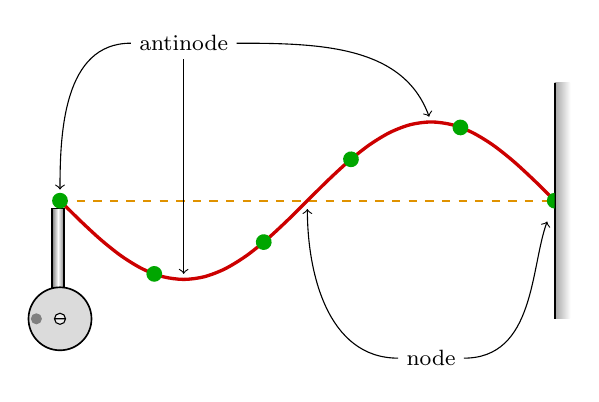
\begin{tikzpicture}
        \footnotesize
        \draw [orx,thick,dashed] (0,0) -- (2*pi,0);

        \filldraw [semithick,left color=gray,right color=gray,middle color=white] (0.05,-0.1) rectangle (-0.1,-1.4);
        \filldraw [semithick,fill=gax!40] (0,-1.5) circle (4mm);
        \fill [gray] (-0.3,-1.5) circle (2pt);
        \fill [gax!20] (0,-1.5) circle (2pt);
        \draw
            (0,-1.5) circle (2pt)
            (-2pt,-1.5) -- ++(4pt,0)
        ;

        \draw [
            rex,very thick,postaction={decorate},
            decoration={
                markings,
                mark=between positions 0.2 and 0.8 step 0.2 with \fill [grx] circle (1mm);
            }
        ] plot[domain=0:2*pi,smooth] (\x,{-sin(\x r)});

        \shade [left color=gax,right color=white] (2*pi,-1.5) rectangle ++(0.2,3);
        \draw [semithick] (2*pi,-1.5) -- ++(0,3);
        \fill [grx]
            (2*pi,0.1) arc[start angle=90,end angle=270,radius=1mm]
            (0,0) circle (1mm)
        ;

        \node at (pi/2,2) {antinode}
            edge [out=180,in=90,->,shorten >=4pt] (0,0)
            edge [out=-90,in=90,->,shorten >=2pt] ({pi/2},-1)
            edge [out=0,in=110,->,shorten >=2pt] ({3*pi/2},1)
        ;
        \node at ({3*pi/2},-2) {node}
            edge [out=180,in=-90,->,shorten >=3pt] (pi,0)
            edge [out=0,in=-110,->,shorten >=8pt] (2*pi,0)
        ;
    \end{tikzpicture}
    \caption{Nodes and antinodes on a standing Wave.}
    \label{fig:standingWaveNodes}
\end{figure}
As can be seen in the right side of Figure \ref{fig:standingWaveNodes} (where the wave evens out), the distance between adjacent nodes and the distance between adjacent antinodes is, in both cases, equal to $\lambda/2$. The distance between a node and its nearest antinode (and vice versa) is $\lambda/4$.



\section{Five Questions}
\begin{enumerate}
    \item In general, what are the boundary conditions of a standing wave?
    \begin{itemize}[label={--}]
        \item Fixed at one end; free or fixed at the other (consider the case in Figure \ref{fig:standingWaveNodes} versus the case of a plucked string on a string instrument).
    \end{itemize}
    \item What is the type of a soundwave (longitudinal or transverse)?
    \begin{itemize}[label={--}]
        \item Longitudinal compression wave.
    \end{itemize}
    \item What is the boundary condition of this specific setup?
    \begin{itemize}[label={--}]
        \item Open-closed.
    \end{itemize}
    \item What is the type of the wave in the spring?
    \begin{itemize}[label={--}]
        \item Longitudinal compression wave.
    \end{itemize}
    \item What is the boundary condition of this setup?
    \begin{itemize}[label={--}]
        \item Open-closed.
    \end{itemize}
\end{enumerate}




\end{document}